\pagestyle{fancy}
\fancyhead[LE,RO]{\thepage}
\fancyhead[RE]{Ap�ndice} %
\fancyhead[LO]{\nouppercase{\rightmark}}
%\fancyhead[RE]{Parte \thepart \rightmark} %

\chapter{Herramientas utilizadas}
\label{apd:herramientasUtilizadas}

\begin{center}
	\begin{longtable}{ m{0.3\textwidth} p{0.7\textwidth} }
		
\includegraphics[align=t,width=0.2\textwidth]{graphs/logo-github}& 
		GitHub es una plataforma para alojar proyectos utilizando el sistema de control de versiones GIT.
		\\ 
		\hline
		 
\includegraphics[align=t,width=0.2\textwidth]{graphs/logo-aws} &  
		 \textit{Amazon Web Services} (AWS) es una colecci�n de servicios web que conjunto forman una plataforma de computaci�n en la nube.
		  \\ 
		  \hline
		   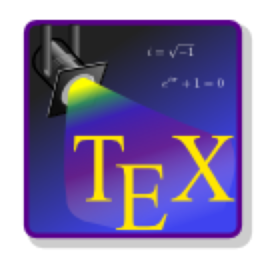
\includegraphics[align=t,width=0.2\textwidth]{graphs/logo-texStudio} &  
		  TeXstudio es un entorno de escritura intregrado para crear documentos LaTeX.
		  \\ 
		  \hline
		  
		  
\includegraphics[align=t,width=0.2\textwidth]{graphs/logo-latex} &  
		  LaTeX es un sistema de composici�n de textos, orientado a la creaci�n de documentos escritos que presenten una alta calidad tipogr�fica.
		  \\ 
		  \hline
		  
		  
\includegraphics[align=t,width=0.2\textwidth]{graphs/logo-illustrator} &  
		  Adobe Illustrator es un editor de gr�ficos vectoriales y est� destinado a la creaci�n art�stica de dibujo y pintura para ilustraci�n. 
		  \\ 
		  \hline
		  
		  
\includegraphics[align=t,width=0.2\textwidth]{graphs/logo-sublime} &  
		  Sublime text es un editor de texto y editor de c�digo fuente.
		  \\ 
		  \hline
		  
		  
\includegraphics[align=t,width=0.2\textwidth]{graphs/logo-node} &  
		  Node.js es un entrono de ejecuci�n para JavaScript construido con el motor de JavaScript V8 de Chrome. 
		  \\ 
		  \hline
		  
		  
\includegraphics[align=t,width=0.2\textwidth]{graphs/logo-angular} &  
		  AngularJS es un \textit{framework} de JavaScript de c�digo abierto, mantenido por Google, que se utiliza para crear y mantener aplicaciones web de una sola p�gina.
		  \\ 
		  \hline
		  
		  
\includegraphics[align=t,width=0.2\textwidth]{graphs/logo-ccs} &  
		  Code Composer Studio es un entorno integrado de desarrollo que soporta los microcontroladores de Texas Instruments. 
		  \\ 
		  \hline
		  
		  
\includegraphics[align=t,width=0.2\textwidth]{graphs/logo-mongo} &  
		  MongoDB es una base de datos NoSQL orientado a documentos, desarrollado bajo el concepto de c�digo abierto.
		  \\ 
		  \hline
		  
		  
\includegraphics[align=t,width=0.2\textwidth]{graphs/logo-raspbian} &  
		  Raspbian es un distribuci�n del sistema operativo GNU/Linux y basado en Debian Jessie para la Raspberry Pi.
		  \\ 
		  \hline

	\end{longtable} 
\end{center}

\chapterend